\section{任务四：无监督疾病判断}
\subsection{问题描述与定义}
训练集中均为正常样本，测试集同时包含正常和患病样本。
目标是从正常训练样本学习正常模式，对新样本输出异常分数$s(\mathbf x)$，分数越大越异常，
当$s(\mathbf x)>\tau$时判为患病（1），否则为正常（0）。这属于正常样本驱动的新颖性检测。

\subsection{数据特点与处理}
训练集1839行，测试集1933行，合计3772行；每行6个脱敏数值特征，无法确定原始医学含义。
测试集1839个正常样本、94个患病样本，患病率约4.86\%，因此仅报告准确率会掩盖异常识别效果。
无缺失或非有限数。训练集有57个重复行，测试集有23个重复行，测试中56行的特征向量也出现于训练。
官方测试集全部保留；特征相同不能确定患者相同，缺少患者标识也无法证明患者级独立性。
对训练数据按相同特征向量分组，以随机种子2026划分拟合子集与正常校准子集，
分别为1476行和363行，两部分没有重复特征组重叠。标准化器仅在拟合子集上学习。

\subsection{方法与阈值设计}
预先指定LOF为主方法，使用35个邻居、novelty=True，以局部密度变化识别正常模式之外的样本。
LOF的新颖性接口仅对未参与拟合的校准集和测试集打分。
固定比较Isolation Forest（300棵树）和RBF One-Class SVM（$\nu=0.05$、gamma=scale），
不根据测试标签选择方法、调参或设置异常比例。所有异常分数均为模型score\_samples取负。

仅使用正常校准分数确定阈值。令校准样本数为$m$，预设$\alpha=0.05$，排序分数为$s_{(1)}\le\cdots\le s_{(m)}$，取
\begin{equation}
 k=\left\lceil(m+1)(1-\alpha)\right\rceil,\qquad\tau=s_{(k)}.
\end{equation}
若$k>m$则阈值为正无穷。本实验$m=363$，使用第346个顺序统计量。
阈值确定后不再用校准集重训，防止分数尺度改变。该阈值控制设计依赖正常校准与未来正常样本可交换的假设；
分布偏移与重复依赖均可能使测试误报率偏离5\%，不能声称无条件保证。

\subsection{实验结果分析}
报告ROC-AUC、平均精确率AP、精确率、召回率、F1和混淆矩阵。
AP使用average\_precision\_score，不等同于梯形积分的PR-AUC。\par
\begin{table}[tbp]\caption{固定模型的测试结果}\label{tab:m3thyroid}\centering
\setlength{\tabcolsep}{3pt}\begin{tabular}{lrrr}
\toprule
Model & AUC & AP & F1\\
\midrule
LOF & 0.9628 & 0.7361 & 0.5498\\
IsolationForest & 0.9810 & 0.7950 & 0.6592\\
OneClassSVM & 0.9765 & 0.7830 & 0.6296\\
\bottomrule\end{tabular}\end{table}
\begin{table}[tbp]\caption{正常校准阈值下的检测效果}\label{tab:m3thyroidthresh}\centering
\setlength{\tabcolsep}{3pt}\begin{tabular}{lrrr}
\toprule
Model & Precision & Recall & FPR\\
\midrule
LOF & 0.4061 & 0.8511 & 0.0636\\
IsolationForest & 0.5087 & 0.9362 & 0.0462\\
OneClassSVM & 0.4830 & 0.9043 & 0.0495\\
\bottomrule\end{tabular}\end{table}
LOF的ROC-AUC为0.9628、AP为0.7361，检出94个患病样本中的80个，漏报14个；1839个正常样本中误报117个。召回率85.11\%，精确率40.61\%，误报率6.36\%。
固定比较的孤立森林在本次测试中表现更好：ROC-AUC为0.9810，F1为0.6592，检出88个患病样本、误报85个正常样本。
保留LOF作为预先指定主方法，同时如实报告这一比较；不能将事后观察到的测试优势称为独立验证后的选择结果。
LOF精确率约四成，表明正常样本中的尾部变化仍造成较多误报，异常分数并非确诊概率。
\begin{figure}[tbp]\centering
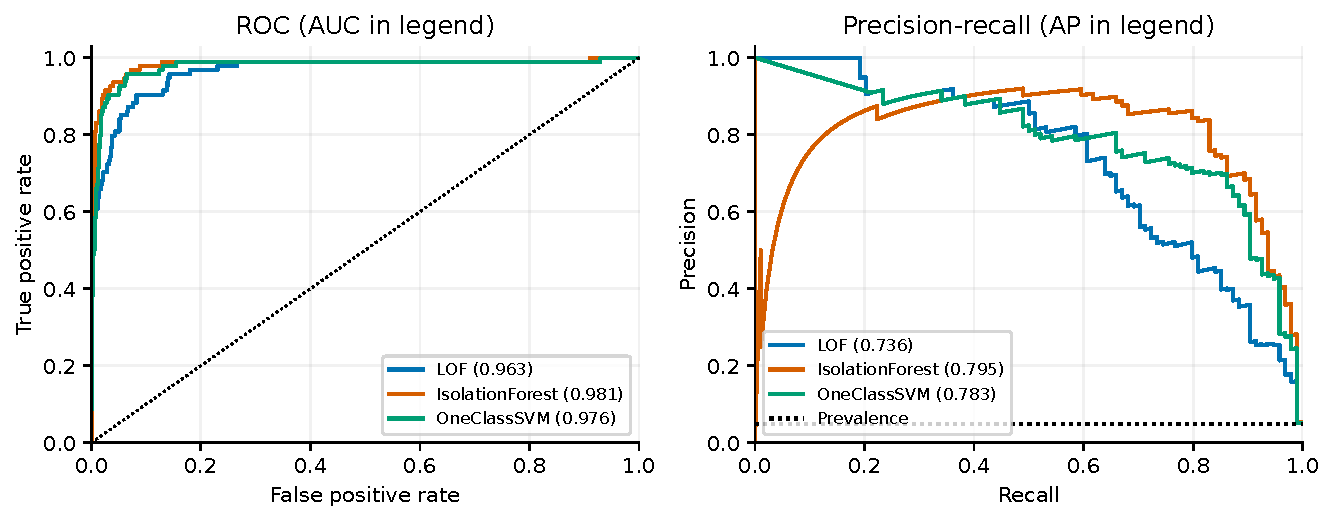
\includegraphics[width=\linewidth]{results/task4/roc_pr.pdf}
\caption{三种固定方法的ROC与PR曲线。}\label{fig:m3roc}
\Description{比较LOF、孤立森林、One-Class SVM在整个测试集的异常排序。}
\end{figure}
\begin{figure}[tbp]\centering
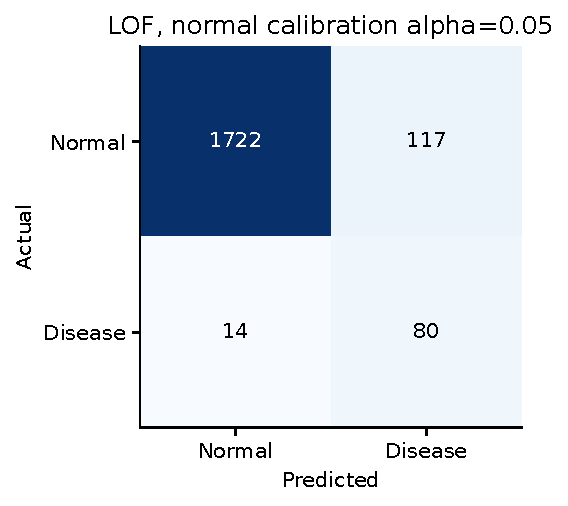
\includegraphics[width=.78\linewidth]{results/task4/confusion_matrix.pdf}
\caption{LOF主方法的混淆矩阵。}\label{fig:m3cm}
\Description{正常1722个判对、117个误报；患病80个检出、14个漏报。}
\end{figure}
\begin{table}[tbp]\caption{LOF预设阈值敏感性（仅作评价）}\label{tab:m3sensitivity}\centering
\setlength{\tabcolsep}{3pt}\begin{tabular}{lrrr}
\toprule
Alpha & Precision & Recall & F1\\
\midrule
0.0100 & 0.7229 & 0.6383 & 0.6780\\
0.0500 & 0.4061 & 0.8511 & 0.5498\\
0.1000 & 0.2622 & 0.9149 & 0.4076\\
\bottomrule\end{tabular}\end{table}
1\%、5\%、10\%三个校准水平提前指定，正式结果仍用5\%，不按测试标签选择最佳F1阈值。
训练样本没有患病标签，无法用有监督交叉验证直接优化患病F1。
此外，输入已被上游脱敏变换，不能核实上游是否使用全数据做标准化；本实现保证新增处理只使用训练子集。
本结果只适用于给定课程数据，尚无跨机构、跨人群验证。
\FloatBarrier
